\subsubsection{Droïde}
\begin{samepage}
	\vspace{4\baselineskip}
	\begin{tabular}{ l l }
		\textbf{Type} 			& Artificiel \\
	   	\textbf{Planète} 		& Multiple \\
	   	\textbf{Language} 		& Binaire \\
	   	\textbf{Orientation} 	& Neutre \\
	\end{tabular}

	\vspace{-11\baselineskip}

	\begin{flushright}
		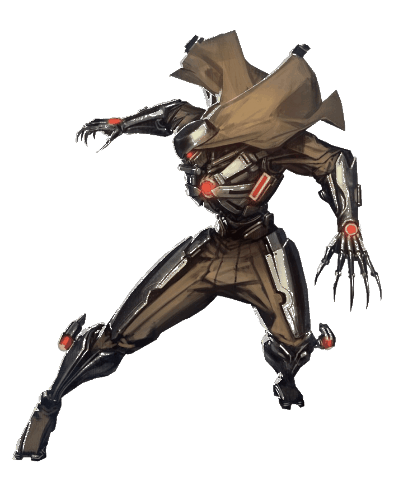
\includegraphics[width=6cm]{img/personnages/races/droide.png}
	\end{flushright}
	\vspace{-2\baselineskip}
\end{samepage}

Les Droïdes ne sont pas une race à proprement parlé mais des entités artificielles créés par d'autres races. Il peuvent être de Combat, de Protocole, de Compagnie, \ldots 
De par leur nature artificielle les Droïdes ne peuvent et ne pourront jamais utiliser la Force, c'est une notion qui leur est totalement étrangère.

\begin{description}[align=left]
\item [Créature artificielle] 	% CAP +2
		Les droides ne ressentent pas la douleur de blessures ou de la perte d'un membre.\\
		\emph{+2 pour se remettre d'un état secoué}\\
		\emph{Pas de bonus aux attaques ciblées}\\
		\emph{Pas de malus de blessure}
\item [Immunisé] 				% CAP +1
		Les maladies et les poisons sont sans effet sur les droides.\\
		\emph{Immunisé}
\item [Ambidextre] 				% CAP +2
		Un droïde ne fait pas de différence entre un membre et un autre, il peut utiliser n'importe lequel indistinctement.\\
		\emph{Ambidextre}
\item [Manque pas d'air] 		% CAP +2
		Les droïdes n'ont pas besoin de respirer, il peuvent stationné dans des lieux dépourvu d'atmosphère. Ils restent cependant sensible à la température.\\
		\emph{Ambidextre}
\item [Pas d'\^Ame] 			% CAP -3
		Il est impossible pour un droïde d'utiliser la force.\\
		\emph{\^Ame <= d6}
		\emph{Compétence Force interdite}
\item [Outsider] 				% CAP -2
		Le droïdes sont considéré comme des servants par les autres espèces, ils n'ont pas de droits et ne sont pas considéré comme faisant parti de la société.\\
		\emph{\'Etrangé}
\end{description}